% ============================================================================
% ex1.tex
% ============================================================================
% Exercício individual da lista.
% Este arquivo deve conter apenas o conteúdo do exercício e, quando desejado,
% sua resolução. Não deve carregar pacotes nem redefinir configurações globais.
%
% Interface adotada neste exemplo:
% - ambiente `exercicio` com identificador textual livre;
% - ambiente `resolucao` para a solução;
% - subseções internas apenas para organizar a exposição.
% ============================================================================

\begin{exercicio}[Problem 1 --- SHG with Gaussian Beams]
Consider the problem of Second Harmonic Generation (SHG) with Gaussian beams. We have discussed how in this case the effective nonlinear coefficient carries an overlap integral that depends on the matching between the interacting fields.

\begin{enumerate}[a)]
    \item Show with a numerical simulation that the Boyd-Kleinman criterion arises from optimizing this overlap integral.
    \item Discuss how the phase mismatch is affected when Gaussian beams are used instead of plane waves.
\end{enumerate}
\end{exercicio}

\begin{resolucao}[Solution]

    \subsection*{(a) Numerical Optimization of the Overlap Integral}

        \paragraph*{Theoretical Framework}
            The analytical treatment of Second Harmonic Generation (SHG) focused by a localized Gaussian beam is detailed in \textbf{Section 2.11 of \authorlinkcite{Boyd}} (4th edition, \textit{Second-Harmonic Generation with Focused Gaussian Beams}). The propagation characteristics and the definition of the confocal parameter follow the standard formulations in \textbf{Section 3.1 of \authorlinkcite{Saleh}} (\textit{Gaussian Beams}).
        
            As demonstrated by Boyd and Kleinman, assuming a fundamental field focused at the center of a nonlinear crystal of length $L$, the total generated second-harmonic power depends directly on the dimensionless efficiency factor $h(\sigma, \xi)$. This factor is defined via the simplified single-integral form (taking advantage of symmetry along the focus):
            \begin{equation}
                h(\sigma, \xi) = \frac{2}{\xi} \left[ \int_{0}^{\xi} \frac{\cos(\sigma \tau) + \tau \sin(\sigma \tau)}{1 + \tau^2} d\tau \right]^2,
                \label{eq:boyd_kleinman}
            \end{equation}
            where the scale parameters are defined as:
            \begin{itemize}
                \item $\xi = L/b$: the dimensionless focusing parameter, related to the crystal length $L$ and the confocal parameter $b = 2 z_R = 2\pi n_1 w_0^2 / \lambda_1$.
                \item $\sigma = \frac{1}{2} b \Delta k$: the normalized wavevector phase mismatch, where $\Delta k = 2k_1 - k_2$.
            \end{itemize}
    
        \paragraph*{Numerical Optimization}
            To find the conditions for maximum conversion efficiency, Eq.~\eqref{eq:boyd_kleinman} was evaluated over a bidimensional grid of the parameters $\xi$ and $\sigma$. The complete algorithm execution and visualization can be found in Appendix~\ref{app:boyd-kleinman-code}.
            
            The numerical maximization yields the classical Boyd-Kleinman optimization criterion:
            \begin{equation}
                \xi_{\mathrm{opt}} \approx 2.84 \quad \text{and} \quad \sigma_{\mathrm{opt}} \approx 0.57.
            \end{equation}
            At this global maximum, the efficiency factor reaches $h(\sigma_{\mathrm{opt}}, \xi_{\mathrm{opt}}) \approx 1.068$. This proves that the highest SHG efficiency occurs when the crystal length is roughly three times the beam's confocal parameter ($L \approx 2.84 b$).

            % === ADICIONE O BLOCO DA FIGURA AQUI ===
            \begin{figure}[H]
                \centering
                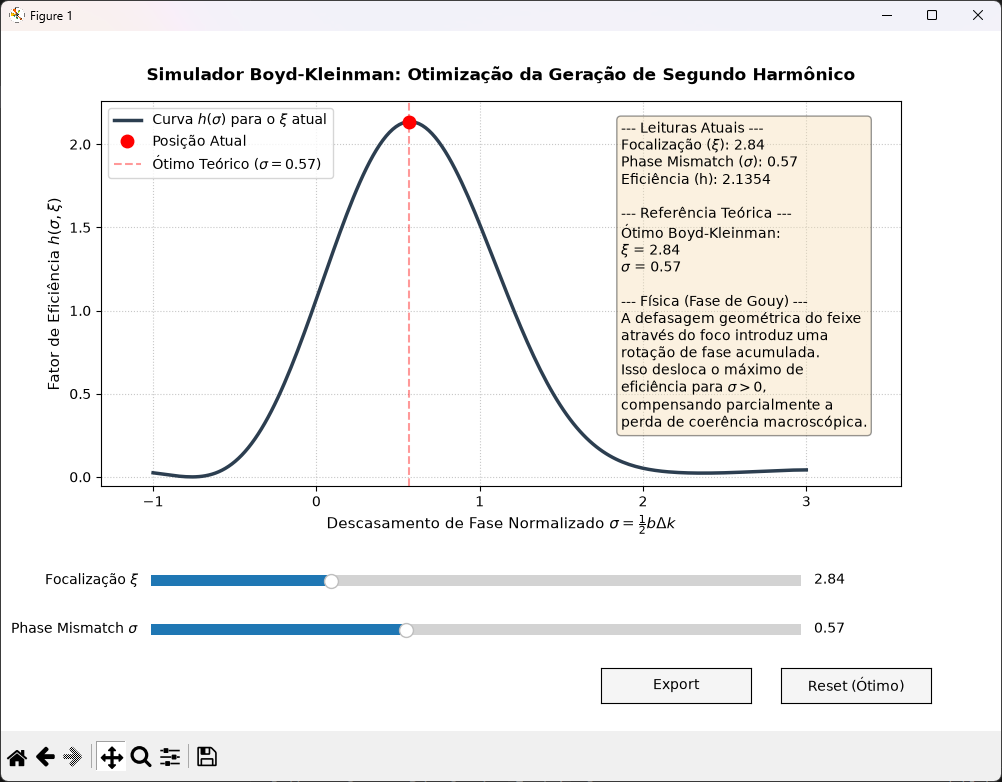
\includegraphics[width=0.75\columnwidth]{Interactive Boyd-Kleinman Simulator.png}
                \caption{Graphical User Interface (GUI) of the interactive script, developed to explore the influence of the Gouy phase shift on the second-harmonic execution in real-time.}
                \label{fig:simulator_gui}
            \end{figure}
            % =======================================

            % === ADICIONE O BLOCO DA FIGURA AQUI ===
            \begin{figure}[H]
                \centering
                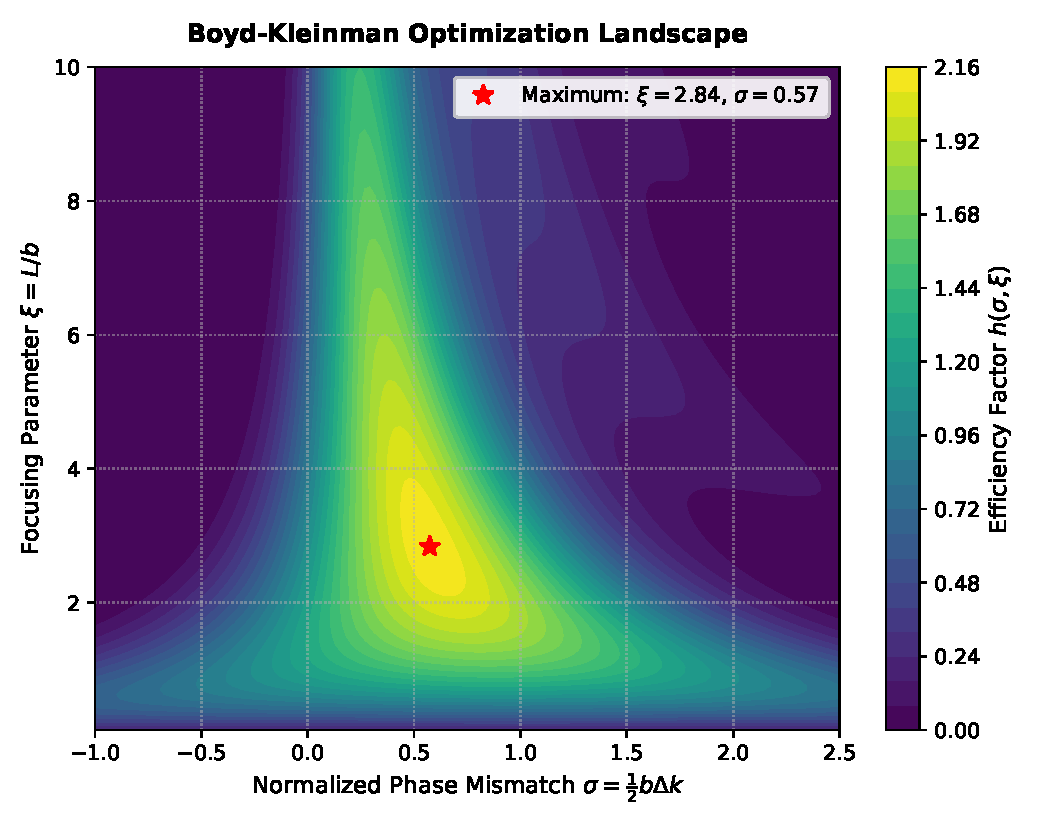
\includegraphics[width=\columnwidth]{boyd_kleinman_plot.pdf}
                \caption{Numerical evaluation of the Boyd-Kleinman factor $h(\sigma, \xi)$ as a function of the normalized phase mismatch $\sigma$ and focusing parameter $\xi$. The red star highlights the global optimum at $\xi \approx 2.84$ and $\sigma \approx 0.57$, where $h_{\max} \approx 1.068$.}
                \label{fig:boyd_kleinman}
            \end{figure}
            % =======================================

    \subsection*{(b) Phase Mismatch: Gaussian Beams vs. Plane Waves}

        The transition from the plane-wave regime to focused Gaussian beams introduces a fundamental shift in the phase-matching requirements.
    
        \paragraph*{Plane-Wave Limit}
            In the limit of weak focusing ($\xi \to 0$), the fields approximate plane waves. As shown in Section~2.2 of \authorlinkcite{Boyd}, the efficiency follows a $\operatorname{sinc}^2(\Delta k L / 2)$ profile, which strictly reaches its maximum at $\Delta k = 0$.
    
        \paragraph*{The Role of the Gouy Phase Shift}
            For focused Gaussian beams ($\xi > 0$), the numerical results show that the optimum mismatch shifts to $\sigma \approx 0.57$, which implies a strictly non-zero material phase mismatch ($\Delta k > 0$). 
            
            Physically, as detailed in Section~3.1 of \authorlinkcite{Saleh}, a Gaussian beam undergoes a total phase advance of $\pi$ radians when passing through its focus, known as the \textbf{Gouy phase shift}. Since the second-order nonlinear polarization is driven by the square of the fundamental field ($P_{\mathrm{NL}} \propto E_1^2$), the driving polarization acquires *twice* the Gouy phase shift ($2\zeta(z)$) compared to a freely propagating wave of the same frequency.
        
            If the material were perfectly phase-matched in the bulk ($\Delta k = 0$), this spatial geometric phase evolution would cause the newly generated second-harmonic wave and the driving polarization to fall out of phase as they cross the focal volume. This phase slip triggers destructive interference, forcing back-conversion of power into the fundamental beam. 
            
            Therefore, to maximize macroscopic energy transfer, a positive material phase mismatch $\Delta k > 0$ must be deliberately introduced. This bulk index mismatch provides a linear phase compensation that exactly cancels out the local geometric phase distortion caused by the Gouy effect near the beam waist.

\end{resolucao}
